\section{Evaluation}
\label{sec:evaluation}

\subsection{Technology stack}
\label{subsec:technology_stack}
Since the project description does not mention specific technologies to be used except for the LaTeX package pgfplots, 
the project team decided to evaluate different technologies for the project by creating working prototypes.
The following chapters describe the evaluation criteria and the results of the evaluation.

\subsubsection{Criteria}
The following criteria are used to decide which technologies should be used for the project:
% TODO: should we add information on how we decided on the criteria and the weights?
\begin{itemize}
    \item Know-how (10\%)
    \item Complexity (20\%)
    \item Usability (30\%)
    \item Distribution (40\%)
\end{itemize}

\subsubsection{Calculation}
The formula for calculating the weighted value of each criterion is:
% TODO: should this be weight * 100 due to the percentages? and should the formular just be the sum for all critera?
\[
v_w = \text{weight} \cdot \frac{\text{evaluation}}{5}
\]
Where $evaluation$ is the scoring between 1--5.
The total score for a given technology is the sum
of weighted values.

\subsubsection{Technologies}
The following technologies were evaluated:
% TODO: should we add information on how we decided to evaluate these technologies?
\begin{itemize}
    \item Kotlin with pdflatex as a dependency
    \item Kotlin bundled with pdflatex
    \item Website with swiftlatex
\end{itemize}

\subsection{Reference LaTeX pgfplots template}
\label{subsec:reference_latex_pgfplots_template}
For building the prototypes we will use the following reference LaTeX template which includes a pgfplots object:~\cite{pgfplots_gallery_sourceforge}

\begin{lstlisting}[caption={Reference LaTeX template with a pgfplots object},label={lst:reference_latex_pgfplots_template},language={[LaTeX]{TeX}}]
\documentclass{article}

\usepackage{siunitx}
\usepackage{tikz} % To generate the plot from csv
\usepackage{pgfplots}

\pgfplotsset{compat=newest} % Allows to place the legend below plot
\usepgfplotslibrary{units} % Allows to enter the units nicely

\sisetup{
  round-mode          = places,
  round-precision     = 2,
}

\begin{document}

\begin{figure}[h!]
  \begin{center}
    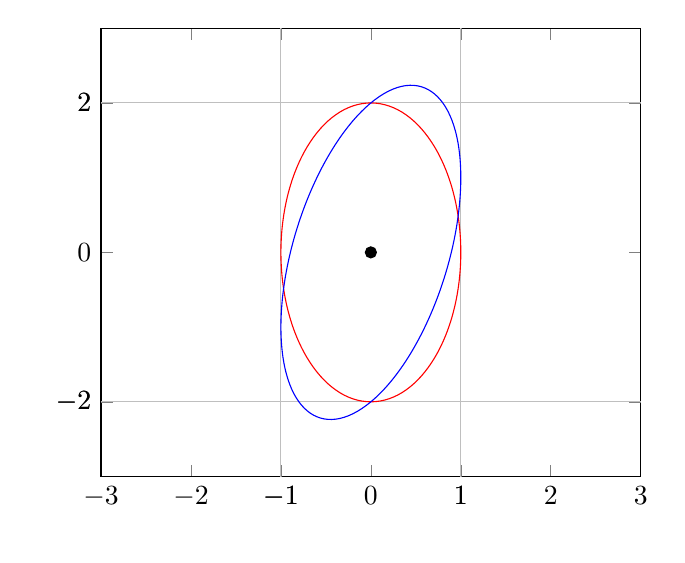
\begin{tikzpicture}
        \begin{axis}[
            xmin=-3,   xmax=3,
            ymin=-3,   ymax=3,
            extra x ticks={-1,1},
            extra y ticks={-2,2},
            extra tick style={grid=major},
        ]
            \draw[red] \pgfextra{
              \pgfpathellipse{\pgfplotspointaxisxy{0}{0}}
                {\pgfplotspointaxisdirectionxy{1}{0}}
                {\pgfplotspointaxisdirectionxy{0}{2}}
              % see also the documentation of
              % 'axis direction cs' which
              % allows a simpler way to draw this ellipse
            };
            \draw[blue] \pgfextra{
              \pgfpathellipse{\pgfplotspointaxisxy{0}{0}}
                {\pgfplotspointaxisdirectionxy{1}{1}}
                {\pgfplotspointaxisdirectionxy{0}{2}}
            };
            \addplot [only marks,mark=*] coordinates { (0,0) };
        \end{axis}
        \end{tikzpicture}
    \caption{My first autogenerated plot.}
  \end{center}
\end{figure}

\end{document}
\end{lstlisting}

\subsubsection{Kotlin minimal - Kotlin with pdflatex as a dependency}
\label{subsubsec:kotlin_minimal}
This prototype uses Kotlin to satisfy platform-independence and invokes the pdflatex binary which is included in the TexLive distribution.
The project team chose to evaluate this technology because it satisfies the base requirements according to the project description and because
the project team is familiar with Kotlin.
Another advantage of this technology is that the distribution of the necessary LaTeX installation and packages is relegated to the user.
This greatly reduces distribution complexity.\newline
An obvious disadvantage of this approach is that the user needs to install TeXLive (and the pgfplots package) on their system, which might be difficult for non-technical users.

\paragraph{Licensing}\mbox{}\newline
This prototype is dependent on both TeXLive and pgfplots.
TeXLive uses a libre license that allows for the free redistribution with or without modifications~\cite{texlive_license} in accordance with the Free Software Foundations's free software definition~\cite{fsf_free_software}.
The pgfplots package uses the GPLv3 license~\cite{pgfplots}.

\paragraph{Evaluation}\mbox{}\newline
\begin{table}[H]
    \centering
    \begin{tabular}{|l|c|c|}
        \hline
        \textbf{Criterion} & \textbf{Evaluation (1-5)} & \textbf{Weighted value} \\
        \hline
        Know-how & 4 & 8 \\
        \hline
        Complexity & 5 & 20 \\
        \hline
        Usability & 1 & 6 \\
        \hline
        Distribution & 5 & 40 \\
        \hline
        \textbf{Total} & n.a & \textbf{74} \\
        \hline
    \end{tabular}
    \caption{Evaluation of Kotlin with pdflatex as a dependency}
    \label{table:kotlin_minimal_evaluation}
\end{table}

\subsubsection{Kotlin bundled - Kotlin bundled with pdflatex}
\label{sec:kotlin_bundled}
Similarily to the prototype in Kotlin minimal~\ref{subsubsec:kotlin_minimal}, this prototype uses Kotlin and invokes the pdflatex binary.
The major difference is that the pdflatex binary is provided alongside
the software.
The advantage of this approach is that the user does not have to install TexLive or any dependencies, greatly improving usability.
However, this comes with the disadvantage
that the complexity of the distribution.
This approach also limits the advantages of using a platform-independent programming language because for every platform there has to be a release
which packages the appropriate binary.

\paragraph{Licensing}\mbox{}\newline
The licensing is equivalent to the licenses of the prototype in Kotlin minimal~\ref{subsubsec:kotlin_minimal}.

\paragraph{Evaluation}\mbox{}\newline
\begin{table}[H]
    \centering
    \begin{tabular}{|l|c|c|}
        \hline
        \textbf{Criterion} & \textbf{Evaluation (1-5)} & \textbf{Weighted value} \\
        \hline
        Know-how & 3 & 6 \\
        \hline
        Complexity & 3 & 12 \\
        \hline
        Usability & 5 & 30 \\
        \hline
        Distribution & 1 & 8 \\
        \hline
        \textbf{Total} & n.a & \textbf{56} \\
        \hline
    \end{tabular}
    \caption{Evaluation of Kotlin bundled with pdflatex}
    \label{table:kotlin_bundled_evaluation}
\end{table}

\subsubsection{Web with swiftlatex}
During the projects initial discussions, which had brainstorm like character, we wondered if we could render latex files directly in the browser, which would have the following benefits:
\begin{itemize}
    \item Providing the functionality as a web application would be probably the easiest and most accessible way for an end user to use the tool.
    \item Introducing the additional constraint of running the application only on the client side, would also avoid any infrastructure service and maintenance cost.
\end{itemize}
After a quick search we found the following open source JavaScript/WebWebassembly project: \href{https://www.swiftlatex.com/}{SwiftLaTeX: WYSIWYG LaTeX Editor for Browsers}
According to their website, the JavaScript/WebWebassembly library has the following characteristics~\cite{swiftlatex_website}:
\begin{itemize}
    \item 100\% Browser - PdfTeX and XeTeX written in 100\% WebAssembly and run in browsers.
    \item Compatibility - Produce exact same output you would get from TexLive or MikTeX\@.
    \item Library Support - Simply include a script tag and use PdfTeX or XeTeX in your own webpage.
    \item WYSIWYG - Support WYSIWYG editing on LaTeX documents using XeTeX engine.
    \item Speed - Run merely 2X slower than native binaries.
    \item Open Source - Completely Open Source. You can find the code on \href{https://github.com/SwiftLaTeX/SwiftLaTeX/}{GitHub}.
\end{itemize}
If the statements on the SwiftLaTeX website hold true, it would neatly full-fill our requirements for building a client side only web application.

\paragraph{Verifying basic functionality}\mbox{}\newline
To make a first feasibility test we can insert our reference LaTeX pgfplots template~\ref{lst:reference_latex_pgfplots_template} into the \href{https://www.swiftlatex.com/\#demo}{SwiftLaTeX Demo tool}.
Even though it took more than one and a half minute to process, we were very surprised that this just worked, see figure~\ref{fig:swiftlatex_demo_rendering_latex_pgfplots_template}:
\begin{figure}[H]
    \centering
    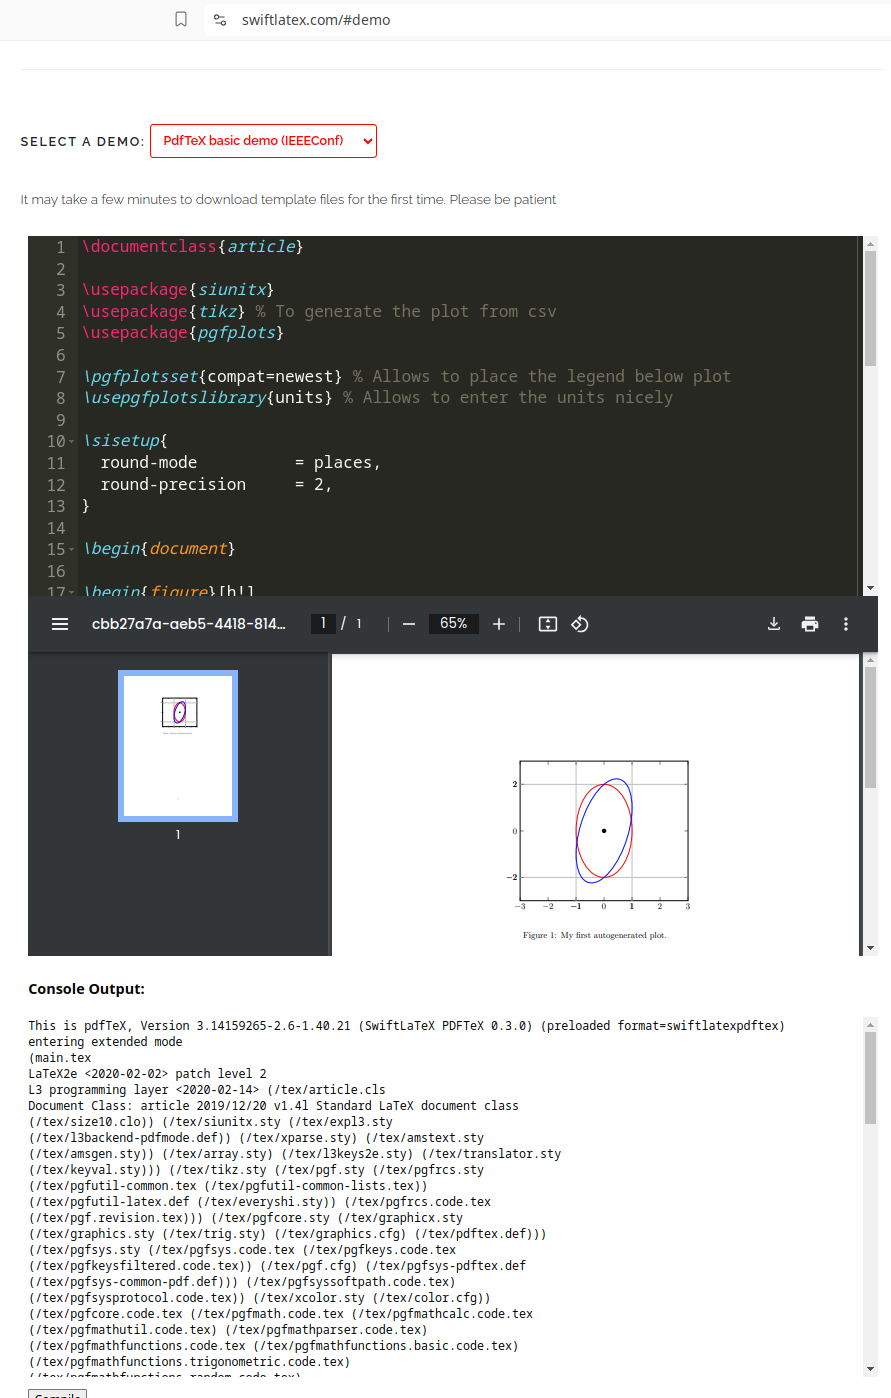
\includegraphics[width=0.5\textwidth]{swiftlatex_demo_pgfplots}
    \caption{Screenshot of the SwiftLaTeX Demo tool rendering the reference LaTeX pgfplots template}
    \label{fig:swiftlatex_demo_rendering_latex_pgfplots_template}
\end{figure}

\paragraph{Investigating dependencies are loaded}\mbox{}\newline
After investigating what actually happens on the page with the browsers developer tools network tab, we saw that SwiftLaTeX will load all dependencies asynchronously via https://texlive2.swiftlatex.com/.
This process and how self-host those files, is documented in the README.md of the SwiftLaTeX GitHub library~\cite{swiftlatex_github_repository}.
As we will be able to specify which LaTeX dependencies our application will use, it would be interesting to download and serve only the files we actually need.
We also saw that the dependencies are loaded sequentially, which we would like to optimize to reduce the pdf generation time.

\paragraph{Local development setup}\mbox{}\newline
To make the same example working on a local machine, we can download the latest release from the GitHub repository: \href{https://github.com/SwiftLaTeX/SwiftLaTeX/releases/tag/v20022022}{Releases 20/02/2022}.
The release contains the website visible at \href{https://www.swiftlatex.com/}{swiftlatex.com} including the compiled WebAssembly files.
As expected, opening the index.html file from the unzipped release folder in a browser will look like the website \href{https://www.swiftlatex.com/}{swiftlatex.com}.
Validating the basic functionality with our reference LaTeX pgfplots template~\ref{lst:reference_latex_pgfplots_template} did not work, as we get the following error message in the JavaScript console:
\begin{lstlisting}[caption={SwiftLaTeX local development setup: JavaScript error message},label={lst:swiftlatex_local_setup_js_error}]
PdfTeXEngine.js:89 Uncaught (in promise) SecurityError: Failed to construct 'Worker': Script at 'file:///home/lukas/Downloads/20-02-2022/swiftlatexpdftex.js' cannot be accessed from origin 'null'.
...
\end{lstlisting}

According to the following \href{https://stackoverflow.com/questions/21408510/chrome-cant-load-web-worker}{stackoverflow question}, Google Chrome does not load web workers when running scripts from local files.
The web worker is required to run WebAssembly, which does all the actual LaTeX to PDF transformation in this prototype.
The easiest solution for this issue is to run a webserver, luckily this is trivial with Python.
We just have to run the following command in the directory of the unpacked SwiftLaTeX release folder:
\begin{lstlisting}[caption={Start a webserver on http://localhost:8000/ with Python},language=bash,label={lst:lstlisting}]
python -m http.server
\end{lstlisting}
Validating the basic functionality with our reference LaTeX pgfplots template~\ref{lst:reference_latex_pgfplots_template} on http://localhost:8000/ works now as expected.

\paragraph{Distribution option 1: Python webserver}\mbox{}\newline
This would be the easiest solution, as it is analog to the local development setup described in the previous paragraph.
But installing Python, downloading the git repository or downloading a release and running the Python web server in the correct directory, requires at least a lot of technical affinity.

\paragraph{Distribution option 2: PyInstaller}\mbox{}\newline
To enhance the end users experience we could build an executable from a Python file with PyInstaller which supports builds for Windows, macOS and Linux.
Even though this solution worked in a quick proof of concept on a linux system, the user would need to find the public GitLab repository and download a release, which contains the latest executables.
Further the user might have security concerns, as downloading an executable from an unknown or untrusted source is really dangerous.

\paragraph{Distribution option 3: GitHub Pages}\mbox{}\newline
After thinking about it, we figured out that we could deploy the tool as a static HTML page to GitHub pages, this would resolve the need of downloading any source code or executable program.
In our opinion this would result in the best user experience, as the user only needs a web browser to access and use the tool.
As this solution was worth exploring, we deployed the prototype with GitHub pages: https://vonal3.github.io/

\paragraph{Licensing}
\begin{itemize}
    \item SwiftLaTeX: \href{https://github.com/SwiftLaTeX/SwiftLaTeX/blob/master/LICENSE}{SwiftLaTeX License}, \href{https://www.gnu.org/licenses/agpl-3.0.en.html}{GNU AFFERO GENERAL PUBLIC LICENSE}
    \item LaTeX: \href{https://www.latex-project.org/lppl.txt}{The LaTeX project public license}
    \item TeXLive: \href{https://www.tug.org/texlive/copying.html}{TeX Live licensing, copying, and redistribution}, \href{https://www.tug.org/texlive/LICENSE.TL}{COPYING CONDITIONS FOR TeX Live}
    \item pgfplots: \href{https://ctan.org/pkg/pgfplots}{https://ctan.org/pkg/pgfplots}, \href{https://www.gnu.org/licenses/gpl-3.0.en.html}{GNU General Public License, version 3 or newer}
\end{itemize}

\paragraph{Evaluation}\mbox{}\newline
\begin{table}[H]
    \centering
    \begin{tabular}{|l|c|c|}
        \hline
        \textbf{Criterion} & \textbf{Evaluation (1-5)} & \textbf{Weighted value} \\
        \hline
        Know-how & 3 & 6 \\
        \hline
        Complexity & 3 & 12 \\
        \hline
        Usability & 4 & 24 \\
        \hline
        Distribution & 5 & 40 \\
        \hline
        \textbf{Total} & n.a & \textbf{82} \\
        \hline
    \end{tabular}
    \caption{Evaluation of SwiftLaTeX JavaScript/WebAssembly library}
    \label{table:swiftlatex_evaluation}
\end{table}

\subsubsection{Chosen Solution}
Using the evaluations given to the selected technologies, the following demonstrates the combined results:
\begin{table}[H]
    \centering
    \begin{tabular}{|l|c|c|}
        \hline
        \textbf{Technology} & \textbf{Total score} \\
        \hline
        Kotlin minimal & 74 \\
        \hline
        Kotlin bundled & 56 \\
        \hline
        Web SwiftLaTeX & 82 \\
        \hline
    \end{tabular}
    \caption{Technology stack evaluation}
    \label{table:technology_evaluation}
\end{table}
In accordance with the table above, the project team decided to use \textbf{Web SwiftLaTeX} with the distribution option 3 \textbf{GitHub Pages}.

\subsection{License}
After evaluating the different possible technologies, the following third party software will be used:
\begin{itemize}
    \item SwiftLaTeX: \href{https://github.com/SwiftLaTeX/SwiftLaTeX/blob/master/LICENSE}{SwiftLaTeX License}, \href{https://www.gnu.org/licenses/agpl-3.0.en.html}{AGPL-3.0}
    \item pgfplots: \href{https://ctan.org/pkg/pgfplots}{https://ctan.org/pkg/pgfplots}{pgfplots}, \href{https://www.gnu.org/licenses/gpl-3.0.en.html}{GPL-3.0}
\end{itemize}
To be conform with the used software, we will also publish our code under the GPL-3.0 licence.